
\chapter{An investigation into the relationship between cardiopulmonary exercise testing and body composition in patients undergoing major pancreatic surgery.}
\label{ch_bodycomp}
\lhead{Chapter \ref{ch_bodycomp}. \emph{CPET and Body Composition}} % This is for the header on each page - perhaps a shortened title
\clearpage
%----------------------------------------------------------------------------------------

\section{Introduction}
Major abdominal surgery especially for pancreatic disease is associated with significant morbidity and mortality. 
Patient selection is as important as identifying surgical treatable pathology in ensuring optimal outcomes \parencite{balthazar_acute_2002}.

\subsection{Role of preoperative CPET}
Cardiopulmonary exercise testing has become a useful tool in the preoperative evaluation and risk assessment/stratification of patients undergoing major thoracic and abdominal surgery. 
A number of studies have shown that poor aerobic fitness demonstrated by a low $\dot{V}_{O_2}$AT or low $\dot{V}_{O_2}$Peak or both was associated with increased morbidity and mortality after major surgery including bariatric \parencite{mccullough_cardiorespiratory_2006}, pancreatic \parencite{ausania_effects_2012}[Chapter \ref{ch_cpet_outcomes}], liver \parencite{epstein_aerobic_2004}, cardiothoracic \parencite{brunelli_risk_2010, campione_oxygen_2010,torchio_exercise_2010} and abdominal aortic aneurysm surgery \parencite{carlisle_mid-term_2007,thompson_cardiopulmonary_2011}. 
It is now routinely used as part of the preoperative work-up to aid in risk assessment and patient selection.
Cardiopulmonary exercise tests also help in identifying patients who may benefit from optimisation and more focussed care before, during and after major pancreatic surgery.
Patients are sometimes denied surgery if their aerobic fitness as determined by cardiopulmonary exercise testing is felt to be too poor based on currently available evidence.

\subsection{Factors affecting aerobic fitness}
Aerobic fitness, as defined by the ability to perform physical exercise, is dependant on and often limited by the ability of the cardiorespiratory and circulatory systems to supply oxygen to skeletal muscles at times of increased demand as well as remove the main end product of aerobic metabolism, $CO_2$. 

Several factors play an important role in meeting this increased metabolic demand. 
These include a normal cardiac and respiratory response to exercise and the oxygen carrying capacity of blood primarily determined by haemoglobin levels. 
Peripherally, an adequate circulatory response to local humoral factors and central autonomic control, capillary density within the skeletal muscle and the ability of skeletal muscle to utilise oxygen, which is in turn determined by mitochondrial mass and function are important factors.

Inadequate or inappropriate response of any of the above mentioned factors will result in overall limitation of oxygen delivery or utilisation and aerobic fitness. 
Cardiopulmonary exercise testing allows the accurate measurement of most of these factors either directly or indirectly during dynamic exercise.
This allows identifying not only limitations in aerobic fitness but also the cause for such limitation. 

A low $\dot{V}_{O_2}$ has universally been attributed to low aerobic fitness due to an inadequate response of the cardiovascular and respiratory systems. 
This is often thought to be due to cardiorespiratory disease, overt or sub-clinical. 
Occasionally, other factors such as anaemia \parencite{agostoni_relationship_2010}, peripheral vascular disease and rarely, mitochondrial diseases \parencite{fernandez_use_2000} have been identified as contributing to low aerobic capacity.

The most common parameters used to quantify perioperative risk in surgical patients are oxygen consumption at the anaerobic threshold ($\dot{V}_{O_2}$AT) and at peak exercise capacity ($\dot{V}_{O_2}$Peak). 
Conventionally these have been reported as per weight ratios (ml/kg/min) to allow comparison between patients. 
However, numerous studies on cardiorespiratory exercise physiology have reported that normalising $\dot{V}_{O_2}$ using total body weight leads to spurious correlation errors unfairly penalising obese subjects \parencite{seltzer_body_1940, tanner_fallacy_1949, toth_examination_1993, batterham_modeling_1999, goran_total_2000, krachler_cardiopulmonary_2014} 

\subsection{Aims}
In chapter \ref{ch_cpet_outcomes}, we reported that low $\dot{V}_{O_2}$AT in patients undergoing pancreaticoduodenectomy was associated with increased incidence of postoperative pancreatic fistula and prolonged hospital stay. 
We also reported that patients with a $\dot{V}_{O_2}$AT less than 10 ml/kg/min were less likely to receive postoperative adjuvant chemotherapy.
In chapter \ref{ch_cpet_jaundice}, while examining the relationship between preoperative clinico-pathological characteristics and cardiopulmonary exercise physiology, we observed that a high body mass index was associated with a low $\dot{V}_{O_2}$AT and $\dot{V}_{O_2}$Peak independent of all other factors. 
Moreover, most of our patients did not have overt cardiac or respiratory comorbidity to explain these findings.

We hypothesised at the end of chapter \ref{ch_cpet_jaundice} that low $\dot{V}_{O_2}$ values in obese patients may be a result of the calculations involved rather than due to true cardiopulmonary dysfunction. 
The aim of the present study was to examine the relationship between cardiopulmonary exercise testing and body composition in patients undergoing pancreaticoduodenectomy in an attempt to explain the strong negative correlation between low $\dot{V}_{O_2}$ and body mass index.

\clearpage
\section{Patients and methods}

\subsection{Patients}
Patients scheduled to undergo pancreaticoduodenectomy for malignant or benign disease involving the head of the pancreas and periampullary region between August 2008 and October 2010 were included in this study. 
All data were recorded in a prospectively maintained database. 
Data was collected on demographics, preoperative clinico-pathological characteristics including blood tests, body mass index, weight, height and the underlying surgical pathology. 
Detailed breath-by-breath data on a variety of physiological and gas-exchange parameters measured at cardiopulmonary exercise testing were also collected from a prospectively maintained database. 
Cardiopulmonary exercise testing methodolgy is discussed in Section \ref{sec:cpx_method} (p\pageref{sec:cpx_parameters})and a description of the parameters measured at cardiopulmonary exercise testing is provided in Section \ref{sec:cpx_parameters} (p\pageref{sec:cpx_parameters}).

\subsection{Calculation of body composition}
\label{sec:bodycomp_calculation}
Computed tomography of the abdomen, performed as part of the routine preoperative staging, was used to calculate body composition based on previously published methods \parencite{bredella_comparison_2010,shen_total_2004}.

%http://regionstraumapro.com/post/16349545265 - Excellent description of CT window width(W) and level/center(C)
The coronal and sagittal reconstructions were used to accurately identify the L3 and L4 vertebrae. 
The CT window width (W) was set at 400 and the level/centre (C) was set at 40. 
This allowed tissue between -160 Hounsfield units and +240 Hounsfield units to be represented in grayscale with adequate contrast between tissues of interest. 
The cross-sectional images at these levels where then exported as grayscale bitmap images. 
The scale in millimetres was included with every image. 
A representative image is shown in Fig. \ref{fig:bc_ct_csa}.
The GNU Image Manipulation Program (GIMP), an advanced, free, open-source, raster graphics editor was used for analysis of all images (www.gimp.org). 
The use of GIMP to analyse cross-sectional imaging for body composition has been described previously although by using a different technique to what has been employed by us \parencite{anblagan_measurement_2013}.

The first step involved converting the bitmap images into JPEG images using lossy compression set at 85\% to minimise sharp transitions between grey areas of very similar colour values. 
This allowed more consistent selection of contiguous areas of similar grey shades. 

The next step involved standardising the scale of all images by dividing the length of the scale on every image by the number of pixels along the scale. 
This resulted in a length in millimetres for each pixel in each image. 
As pixels on a CT image are square, the area of each pixel was calculated as a square of its length. 

The Fuzzy Select (Magic Wand) tool was used to select contiguous areas of similar colour while simultaneously confirming visually that the correct anatomical structures had been selected without overspill into adjoining unwanted tissue areas. 
The number of pixels within the selection was obtained using the 'Histogram' dialog window and entered into a Microsoft Excel spreadsheet.
The area was calculated by multiplying the number of pixels by the area of each pixel.

\textbf{Selecting tissue compartments}:

The sequence of steps followed to calculate the area of each tissue compartment is depicted in Fig. \ref{fig:bc_ct_gimp} on p\pageref{fig:bc_ct_gimp}. 
The total cross-sectional area of the abdomen at the level of L3/L4 was calculated by first selecting all the empty space outside the image followed by inverting this selection. 
This is depicted in Fig. \ref{fig:bc_ct_csa}. 
Subcutaneous fat in the image was selected using the Fuzzy Select tool (if necessary by choosing multiple times and removing any unnecessary areas) as depicted in Fig. \ref{fig:bc_ct_sat}. 
The same process was repeated for visceral adipose tissue and skeletal muscle as depicted in Fig. \ref{fig:bc_ct_vat} and Fig. \ref{fig:bc_ct_sm} respectively. 
Every selection was visually confirmed for anatomical accuracy by using the layer selection tool to inspect the area under selection as shown in the insets in each of the images.
%CT slices images x 4
\begin{figure}[htbp]
	\centering
	\begin{subfigure}{0.45\textwidth}
		\centering
		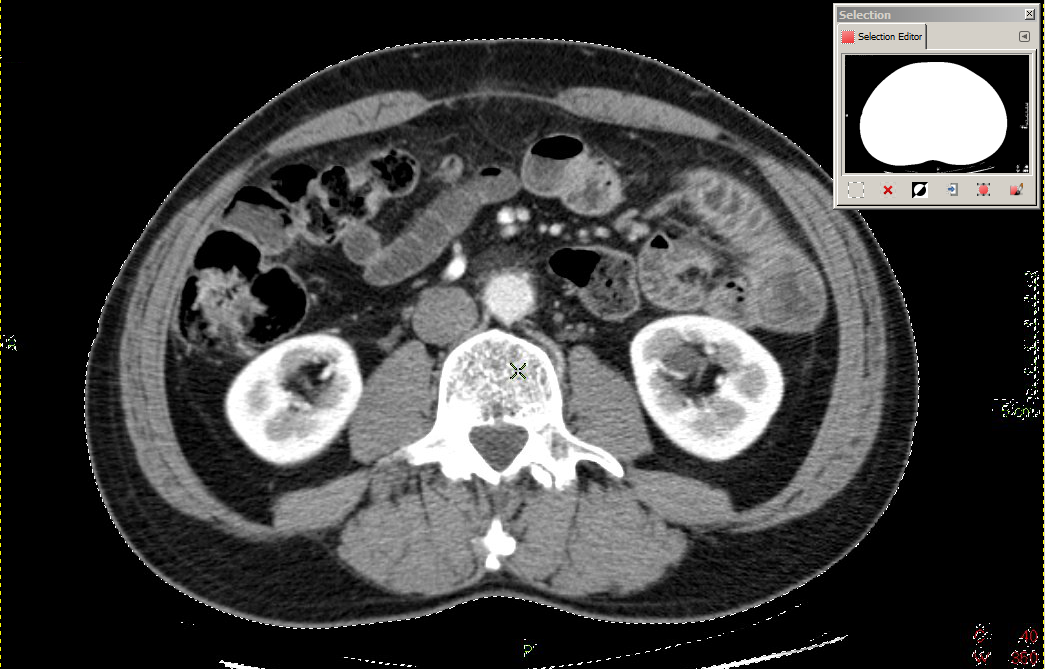
\includegraphics[width=\textwidth]{Figures/bc_ct_csa}
		\caption{Total Cross-sectional Area}
		\label{fig:bc_ct_csa}
	\end{subfigure}
	\begin{subfigure}{0.45\textwidth}
		\centering
		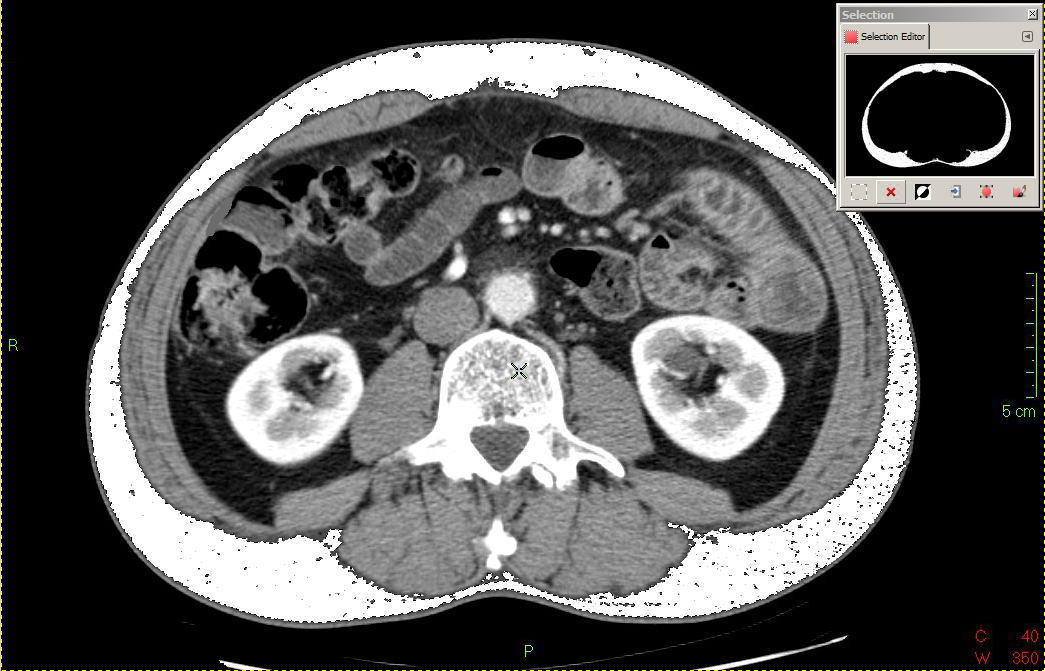
\includegraphics[width=\textwidth]{Figures/bc_ct_sat}
		\caption{Subcutaneous Adipose Tissue$^*$}
		\label{fig:bc_ct_sat}
	\end{subfigure}
	\hfill
	\begin{subfigure}{0.45\textwidth}
		\centering
		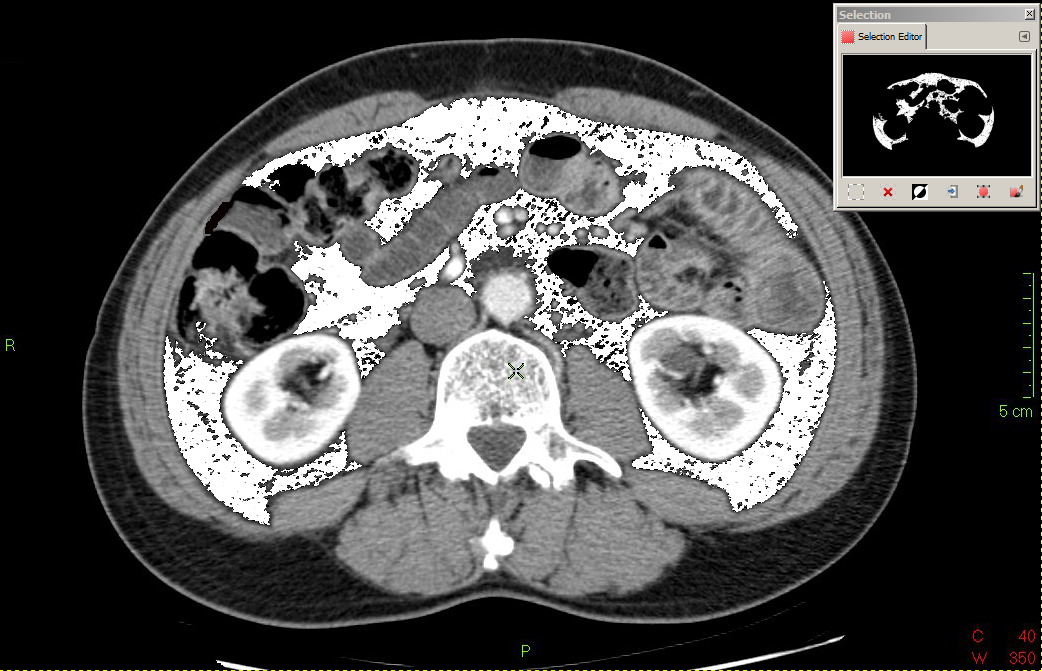
\includegraphics[width=\textwidth]{Figures/bc_ct_vat}
		\caption{Visceral Adipose Tissue$^*$}
		\label{fig:bc_ct_vat}
	\end{subfigure}
	\begin{subfigure}{0.45\textwidth}
		\centering
		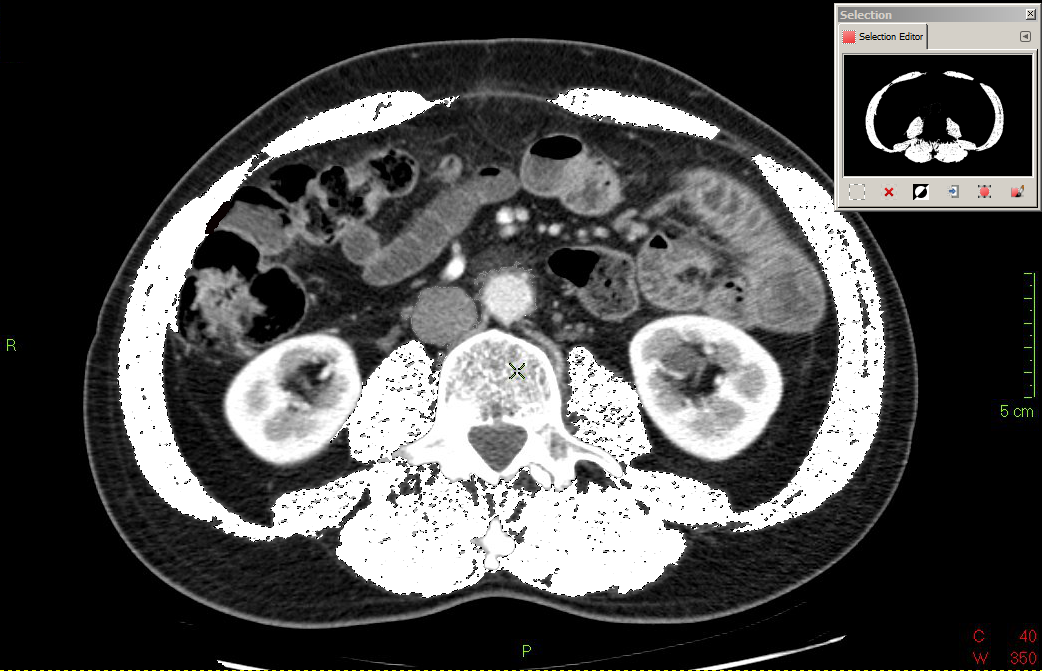
\includegraphics[width=\textwidth]{Figures/bc_ct_sm}
		\caption{Skeletal Muscle$^*$}
		\label{fig:bc_ct_sm}
	\end{subfigure}
	
	\caption{Selection of components of body composition from CT images using GIMP.}($^*$ The selected area has been removed for representation purposes. 
The inset confirms the area selected.)
	\label{fig:bc_ct_gimp}
	
\end{figure}

\subsection{Cardiopulmonary exercise testing}
All patients performed cardiopulmonary exercise testing on a cycle ergometer as described in Section \ref{sec:cpx_method}. 
Raw data of all breath-by-breath parameters averaged every 10 seconds was collected for analysis. 
The first three minutes of the recorded data were during the rest period when the patients were on the exercise bike but did not exercise. 
The average of each parameter measured between the first and second minute (6 readings) was treated as the rest value. 
Anaerobic threshold was identified using previously established methods \parencite{beaver_new_1986,sue_metabolic_1988} and all corresponding parameters at this point were recorded. 
Peak exercise was identified by the maximum oxygen consumption recorded towards the end of the exercise period and all other parameters recorded at this point were considered as peak exercise values.

In order to distinguish between absolute values and values scaled to total body weight, the terms `absolute $\dot{V}_{O_2}$' and `corrected $\dot{V}_{O_2}$' are used throughout this chapter. 
When $\dot{V}_{O_2}$ has been scaled to an alternate factor, this is stated clearly. 

\subsection{Estimation of lean body mass}
\label{sec:elbm}
Estimated lean body mass (eLBM) was calculated using the Boer formula \parencite{boer_estimated_1984} as shown below.
\begin{equation} \label{eq:elbm_men}
	Men:\ eLBM = 0.407 \times weight(kg) + 0.267 \times height(cm) - 19
\end{equation}
\begin{equation} \label{eq:elbm_women}
	Women:\ eLBM = 0.252 \times weight(kg) + 0.473 \times height(cm) - 48.3
\end{equation}

\subsection{Statistics} 
Comparison between body composition and cardiopulmonary exercise testing parameters was done using Partial correlations controlling for the effect of sex (and/or age). 
The relationship between body composition and preoperative clinico-pathological characteristics (as categorical variables) was analysed using non-parametric tests. 
The Mann-Whitney U test for variables with two categories or the Kruskal-Wallis test for variables with more than two categories. 
Previously established thresholds were used for categorising continuous variables where applicable. 
All reported p-values are two-sided. 
The level of significance was set at $p<0.05$.
SPSS software (Version 22.0; SPSS Inc., Chicago, IL, USA) was used to perform statistical analysis.

\clearpage
\section{Results}

\subsection{Body composition and clinico-pathological characteristics}
Eighty-two patients (52 male) were included in the study. 
The clinico-pathological characteristics of the study patients and their relationship to body composition is shown in Table \ref{table:bc_clinical} on page \pageref{table:bc_clinical}. 
There were several significant associations between clinico-pathological variables and body composition as shown in this table. 
Females had a greater area of subcutaneous adipose tissue (223.9 versus 141.6 cm$^2$, p$<$0.001) but less visceral adipose tissue (79.1 versus 174.9 cm$^2$, p$<$0.001).
However, there was no difference in the total adipose tissue area between men and women (316.6 versus 303.0 cm$^2$, p=0.665).
Skeletal muscle area was greater in males than in females (141.3 versus 99.7 cm$^2$).

Patients from more deprived areas of Scotland as defined by the Scottish Index of Multiple Deprivation (SIMD) had a greater amount of subcutaneous adipose tissue (p=0.041) but no difference in the other body composition parameters.
Hypoalbuminemia was associated with less visceral adipose tissue (p=0.013) and less skeletal muscle area that did not reach statistical significance (p=0.054). 
Anaemia (haemoglobin $<$ 12 g/dl) was associated with increased adiposity in the subcutaneous plane and reduced skeletal muscle area. 
	%%Table 1
\begin{sidewaystable}[p]
 \caption{Body composition parameters distributed by sex in patients undergoing major pancreatic surgery.}
 \label{table:bc_sex_specific_distrib}
 \renewcommand{\arraystretch}{1.2} %Increases space between rows
 %\setlength{\tabcolsep}{9pt} %sets the space between columns
 \centering
 \begin{tabular}{|l|c c c | c c c |c|}
 	\hline
 	                                                  &       \multicolumn{3}{c}{Male}       &       \multicolumn{3}{c}{Female}       & p        \\
 	                                                  &  Mean (SD)   & Range       & n(\%)   & Mean (SD)    & Range       & n(\%)     &  \\ \hline
 	\textbf{Body Mass Index}                          &  26.1 (3.9)  & 18.7-37.6   &         & 24.9 (3.5)   & 18.4-32.4   &           &  \\
 	Underweight ($<$18.5)                             &              &             & 0 (0)   &              &             & 1 (3)     &  \\
 	Normal (18.5-24.9)                                &              &             & 23 (44) &              &             & 15 (50)   &  \\
 	Overweight (25.0-29.9)                            &              &             & 20 (39) &              &             & 11 (37)   &  \\
 	Obese ($>$30)                                     &              &             & 9 (17)  &              &             & 3 (10)    &  \\ \hline
 	\textbf{Total fat index (cm$^2$/m$^2$)}           & 106.7 (55.7) & 30.4-319.1  &         & 118.8 (65.7) & 24.3-357.7  &           & 0.408    \\
 	Sex-specific tertile "Low"                        & 51.4 (14.9)  & 30.4-74.8   & 17 (33) & 61.6 (25.6)  & 24.3-89.6   & 10 (33.3) &  \\
 	Sex-specific tertile "Medium”                     & 98.9 (17.5)  & 75.1-129.1  & 17 (33) & 111.2 (11.1) & 93.0-124.7  & 10 (33.3) &  \\
 	Sex-specific tertile "High”                       & 166.2 (44.2) & 130.3-319.1 & 18 (34) & 183.6 (69.2) & 125.1-357.7 & 10 (33.3) &  \\ \hline
 	\textbf{Subcutaneous fat index (cm$^2$/m$^2$) }   & 47.4 (31.7)  & 13.7-202.8  &         & 87.8 (51.4)  & 20.8-293.7  &           & $<$0.001 \\
 	Sex-specific tertile "Low”                        &  22.6 (6.8)  & 13.7-31.5   & 17 (33) & 49.5 (17.5)  & 20.8-68.3   & 10 (33.3) &  \\
 	Sex-specific tertile "Medium”                     &  40.4 (5.0)  & 32.2-49.1   & 17 (33) & 77.5 (5.2)   & 71.1-89.3   & 10 (33.3) &  \\
 	Sex-specific tertile "High”                       & 77.5 (36.4)  & 50.2-202.8  & 18 (34) & 136.4 (61.7) & 89.5-293.7  & 10 (33.3) &  \\ \hline
 	\textbf{Visceral fat index (cm$^2$/m$^2$)}        & 59.3 (34.6)  & 9.1-164.4   &         & 31.0 (20.7)  & 0.9-82.5    &           & $<$0.001 \\
 	Sex-specific tertile "Low”                        &  23.0 (8.9)  & 9.1-38.1    & 17 (33) & 10.4 (7.9)   & 0.9-20.2    & 10 (33.3) &  \\
 	Sex-specific tertile "Medium”                     & 54.8 (12.7)  & 38.4-77.4   & 17 (33) & 26.9 (5.8)   & 20.8-35.5   & 10 (33.3) &  \\
 	Sex-specific tertile "High”                       & 97.7 (21.6)  & 79.3-164.4  & 18 (34) & 55.8 (10.9)  & 46.7-82.5   & 10 (33.3) &  \\ \hline
 	\textbf{Skeletal muscle fat index (cm$^2$/m$^2$)} &  47.9 (8.8)  & 30.2-72.5   &         & 38.8 (5.3)   & 24.9-49.9   &           & $<$0.001 \\
 	Sex-specific tertile "Low”                        &  38.5 (4.2)  & 30.2-43.8   & 17 (33) & 32.9 (3.3)   & 24.9-36.2   & 10 (33.3) &  \\
 	Sex-specific tertile "Medium”                     &  47.8 (2.1)  & 44.5-51.1   & 17 (33) & 39.5 (1.0)   & 37.8-40.6   & 10 (33.3) &  \\
 	Sex-specific tertile "High”                       &  56.9 (6.1)  & 51.3-72.5   & 18 (34) & 43.9 (3.4)   & 40.9-49.9   & 10 (33.3) &  \\ \hline
 \end{tabular}
\end{sidewaystable}
	%%Table 1
\begin{sidewaystable}[p]
	\tiny
	\caption{The relationship between body composition and clinico-pathological characteristics of patients undergoing major pancreatic surgery.}
	\label{table:bc_clinical}
	%\renewcommand{\arraystretch}{1.2} %Increases space between rows
	\setlength{\tabcolsep}{9pt} %sets the space between columns
	\centering
	\begin{tabular}{|l l| c c | c c| c c | c c |c c |}
		                    &           & \multicolumn{2}{c}{Body Mass} & \multicolumn{2}{c}{Total fat} & \multicolumn{2}{c}{Subcutaneous fat } & \multicolumn{2}{c}{Visceral fat} & \multicolumn{2}{c}{Skeletal Muscle} \\
		                    &           & index           & p           & index        & p              & index        & p                      & index        & p                 & index        & p                    \\
		                    &           & norm/Over/Obese &             & low/med/high &                & low/med/high &                        & low/med/high &                   & low/med/high &  \\
		Age                 & $<$65     & 19/10/6         & 0.752       & 13/12/10     & 0.353          & 16/7/12      & 0.230                  & 11/14/10     & 0.699             & 12/8/15      & 0.486                \\
		                    & $\geq$65  & 19/21/6         &             & 14/15/18     &                & 11/20/16     &                        & 16/13/18     &                   & 15/19/13     &  \\
		SMID                & 0         & 27/18/4         & 0.053       & 22/11/16     & 0.066          & 19/15/15     & 0.211                  & 21/13/15     & 0.094             & 22/12/15     & 0.129                \\
		                    & 1         & 6/8/6           &             & 3/9/9        &                & 5/7/9        &                        & 3/10/8       &                   & 4/9/8        &  \\
		Pathology           & Benign    & 7/2/1           & 0.239       & 5/1/4        & 0.646          & 4/4/2        & 0.385                  & 4/2/4        & 0.960             & 7/1/2        & 0.036                \\
		                    & Malignant & 31/29/11        &             & 22/26/24     &                & 23/23/26     &                        & 23/25/24     &                   & 20/26/26     &  \\
		$\dot{V}_{O_2}$AT   & $\geq$ 10 & 23/12/3         & 0.010       & 20/10/9      & 0.002          & 16/13/10     & 0.082                  & 17/14/8      & 0.011             & 15/11/13     & 0.506                \\
		                    & $<$ 10    & 15/19/9         &             & 7/17/19      &                & 11/14/18     &                        & 10/13/20     &                   & 12/16/15     &  \\
		$\dot{V}_{O_2}$Peak & $\geq$ 16 & 21/12/1         & 0.002       & 18/11/6      & 0.001          & 14/14/7      & 0.044                  & 17/13/5      & 0.001             & 13/10/12     & 0.699                \\
		                    & $<$ 16    & 17/19/11        &             & 9/16/22      &                & 13/13/21     &                        & 10/14/23     &                   & 14/17/16     &  \\
		CRP                 & $\leq$ 10 & 24/18/7         & 0.556       & 16/17/17     & 0.915          & 18/18/14     & 0.205                  & 15/17/18     & 0.511             & 17/15/18     & 0.915                \\
		                    & $>$ 10    & 14/13/5         &             & 11/10/11     &                & 9/9/14       &                        & 12/10/10     &                   & 10/12/10     &  \\
		Albumin             & $\geq$ 35 & 14/14/4         & 0.777       & 10/8/14      & 0.321          & 9/14/9       & 0.915                  & 9/9/14       & 0.205             & 13/9/10      & 0.352                \\
		                    & $<$ 35    & 24/17/8         &             & 17/19/14     &                & 18/13/19     &                        & 18/18/14     &                   & 14/18/18     &  \\
		Haemglobin          & $\geq$ 12 & 26/16/8         & 0.777       & 20/13/17     & 0.321          & 15/21/14     & 0.658                  & 17/17/16     & 0.658             & 16/15/19     & 0.511                \\
		                    & $<$ 12    & 12/15/4         &             & 7/14/11      &                & 12/6/14      &                        & 10/10/12     &                   & 11/12/9      &  \\
		PPS                 & $\leq$ 14 & 16/18/7         & 0.136       & 12/12/17     & 0.228          & 8/19/14      & 0.140                  & 14/12/15     & 0.893             & 13/15/13     & 0.893                \\
		                    & $>$ 14    & 22/13/5         &             & 15/15/11     &                & 19/8/14      &                        & 13/15/13     &                   & 14/12/15     &  \\
		Cardiac             & No        & 25/10/7         & 0.112       & 18/13/12     & 0.080          & 17/14/12     & 0.138                  & 20/10/13     & 0.043             & 21/12/10     & 0.002                \\
		disease             & Yes       & 13/21/5         &             & 9/14/16      &                & 10/13/16     &                        & 7/17/15      &                   & 6/15/18      &  \\
		Respiratory         & No        & 32/27/12        & 0.239       & 22/24/26     & 0.201          & 22/24/26     & 0.201                  & 23/23/26     & 0.385             & 25/23/24     & 0.442                \\
		disease             & Yes       & 6/4/0           &             & 5/3/2        &                & 5/3/2        &                        & 4/4/2        &                   & 2/4/4        &
	\end{tabular}
\end{sidewaystable}

		
	%Table 1
\begin{sidewaystable}[p]
\caption{The relationship between body composition and clinico-pathological characteristics of patients undergoing major pancreatic surgery.}
\label{table:bc_clinical}
\centering
\begin{tabular}{l c c | c c c | c c c | c c c}
	           &           &    & CSA   &       &          & TAT   &       &          & SM    &      &  \\
	           &           & n  & Mean  & SD    & p        & Mean  & SD    & p        & Mean  & SD   & p        \\ \hline
	Age        & $<$ 65    & 35 & 688.6 & 192.8 & 0.386    & 297.0 & 178.5 & 0.309    & 128.7 & 29.4 & 0.590    \\
	           & $\geq$ 65 & 47 & 704.3 & 150.6 &          & 322.7 & 156.6 &          & 124.1 & 31.3 &  \\
	Gender     & M         & 52 & 738.4 & 171.2 & $<$0.001 & 316.6 & 170.8 & 0.665    & 141.3 & 26.1 & $<$0.001 \\
	           & F         & 30 & 626.9 & 141.6 &          & 303.0 & 159.3 &          & 99.7  & 15.6 &  \\
	BMI        & $\leq$ 25 & 39 & 579.9 & 103.6 & $<$0.001 & 205.9 & 97.0  & $<$0.001 & 114.6 & 26.6 & 0.002    \\
	           & 25-30     & 31 & 754.0 & 109.4 &          & 350.6 & 99.6  &          & 136.0 & 30.4 &  \\
	           & $>$ 30    & 12 & 934.6 & 145.4 &          & 554.6 & 185.9 &          & 137.6 & 30.9 &  \\
	SMID       & $>$ 3     & 49 & 684.4 & 163.1 & 0.366    & 288.7 & 175.5 & 0.040    & 123.2 & 31.6 & 0.380    \\
	           & $\leq$ 3  & 21 & 718.5 & 187.2 &          & 365.7 & 165.0 &          & 128.2 & 31.9 &  \\
	Pathology  & Benign    & 10 & 737.9 & 228.4 & 0.766    & 352.8 & 278.1 & 0.955    & 122.4 & 24.0 & 0.788    \\
	           & Malignant & 72 & 692.0 & 160.3 &          & 305.9 & 145.9 &          & 126.6 & 31.3 &  \\
	VO$_2$AT   & $\geq$ 10 & 39 & 659.8 & 173.1 & 0.035    & 257.2 & 144.3 & 0.003    & 131.5 & 33.2 & 0.111    \\
	           & $<$ 10    & 43 & 731.9 & 159.4 &          & 361.0 & 170.1 &          & 121.2 & 27.1 &  \\
	VO$_2$Peak & $\geq$ 16 & 35 & 663.8 & 172.5 & 0.112    & 249.3 & 143.0 & 0.002    & 136.9 & 31.1 & $<$0.001 \\
	           & $<$ 16    & 47 & 722.8 & 163.6 &          & 358.1 & 167.7 &          & 118.0 & 27.5 &  \\
	CRP        & $\leq$ 10 & 50 & 691.4 & 183.1 & 0.512    & 303.7 & 145.2 & 0.985    & 128.7 & 33.5 & 0.392    \\
	           & $>$ 10    & 32 & 707.3 & 146.4 &          & 324.0 & 195.6 &          & 122.0 & 24.7 &  \\
	Albumin    & $\geq$ 35 & 32 & 743.8 & 173.5 & 0.062    & 339.4 & 179.3 & 0.213    & 134.5 & 34.1 & 0.054    \\
	           & $<$ 35    & 50 & 668.1 & 160.8 &          & 293.8 & 155.8 &          & 120.7 & 26.7 &  \\
	Hb         & $\geq$ 12 & 50 & 698.0 & 172.4 & 0.725    & 292.5 & 145.4 & 0.372    & 133.4 & 32.1 & 0.005    \\
	           & $<$ 12    & 32 & 697.1 & 166.2 &          & 341.5 & 192.2 &          & 114.6 & 23.6 &  \\
	PPS        & $\leq$ 14 & 41 & 708.7 & 169.8 & 0.444    & 323.2 & 155.0 & 0.347    & 129.8 & 34.5 & 0.351    \\
	           & $>$ 14    & 41 & 686.5 & 169.5 &          & 300.0 & 177.1 &          & 122.4 & 25.5 &  \\
	Cardiac    & No        & 43 & 675.2 & 185.7 & 0.109    & 305.5 & 195.5 & 0.208    & 120.7 & 33.0 & 0.047    \\
	disease    & Yes       & 39 & 722.3 & 146.8 &          & 318.4 & 127.6 &          & 132.0 & 26.4 &  \\
	Resp.      & No        & 72 & 704.8 & 170.8 & 0.269    & 319.0 & 169.3 & 0.342    & 125.8 & 30.5 & 0.810    \\
	disease    & Yes       & 10 & 646.1 & 153.2 &          & 258.3 & 133.3 &          & 128.0 & 30.9 &
\end{tabular}
\end{sidewaystable}

\subsection{Body composition vs. BMI/sex}
The body composition differences between male and female patients with increasing body mass index is shown in Figure \ref{fig:bc_gender_bmi} on page \pageref{fig:bc_gender_bmi}. 
There were significant differences in the proportion of subcutaneous adipose tissue versus visceral adipose tissue between males and females. 
Men generally had less subcutaneous fat but more visceral fat and skeletal muscle areas. 
However, the proportion of skeletal muscle in both males and females decreased significantly with increasing body mass index.

\begin{figure}[h]
	\centering
	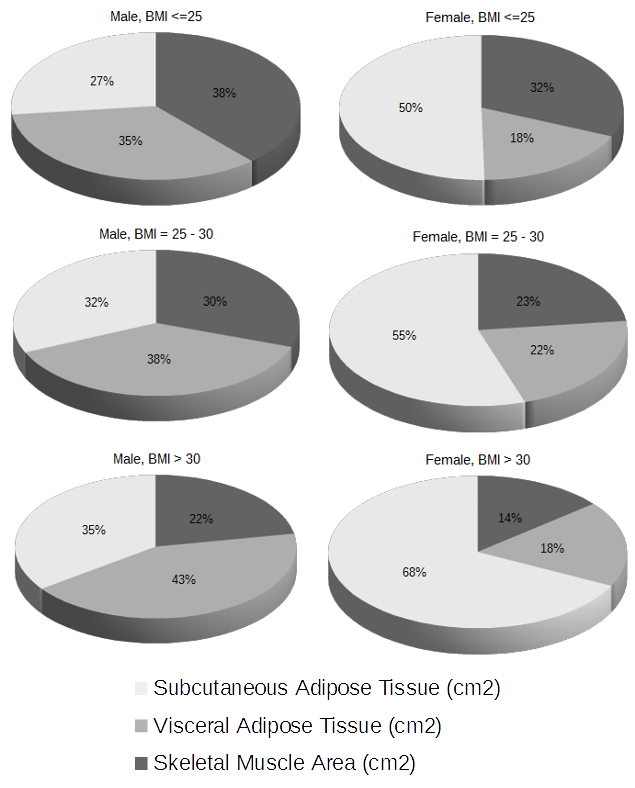
\includegraphics[width=0.8\textwidth]{Figures/bc_gender_bmi_pie}
	\caption{Differences in body composition according to sex and body mass index.}
	\label{fig:bc_gender_bmi}
\end{figure}

The proportion of skeletal muscle area decreases from 38\% in male patients with normal BMI to 22\% in males who are obese. 
There was a greater decrease in the proportion of skeletal muscle in females with increasing BMI, with skeletal muscle area decreasing from 32\% in females with normal BMI to 14\% in obese females. 
The higher weight in the high BMI patients was due to a disproportionate increase in adipose tissue rather than skeletal muscle. 
Moreover, the distribution of the adipose tissue differed between males and females.
Visceral adipose tissue contributed more to weight in obese males (43\% VAT vs. 35\% SAT) while obese females had a greater proportion of subcutaneous adipose tissue than visceral adipose tissue (18\% VAT vs. 68\% SAT).

\subsection{Body composition vs. pulmonary function tests}

Partial correlation analysis was performed to study the relationship between pulmonary function tests and body composition. 
It has been well-established in previous studies that pulmonary function tests are correlated with age and gender and the analysis was therefore adjusted for these two variables. 
Forced Vital Capacity (FVC, litres), Forced Expiratory Volume in 1 second (FEV1, litres) and the ratio FEV1/FVC (Tiffeneau-Pinelli index,\%) were compared against the various components of body composition. 
Both FVC and FEV1 were positively correlated with skeletal muscle area but not with adipose tissue area or total cross-sectional area. 
FEV1/FVC was not correlated with any of the body composition components. 

This would indicate that pulmonary function was dependent on skeletal muscle area while FEV1/FVC, a calculated index to quantify restrictive or obstructive lung disease, was not associated with skeletal muscle area. 
These results are shown in Table \ref{table:bc_cpet} on page \pageref{table:bc_cpet}.

\subsection{Body composition vs. exercise load}

\begin{figure}[htb]
	\centering
	\begin{subfigure}[b]{0.45\textwidth}
		\centering
		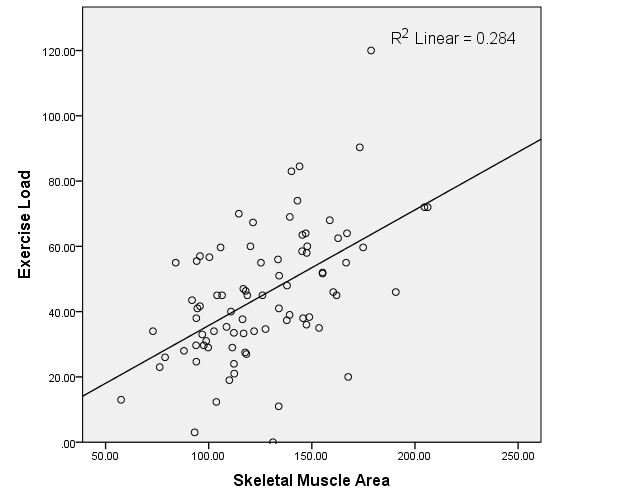
\includegraphics[width=\textwidth]{Figures/bc_scatter_atLoad_skeletal}
		\caption{Anaerobic Threshold}
		\label{fig:bc_at_load_vs_sm}
	\end{subfigure}
	\hfill
	\begin{subfigure}[b]{0.45\textwidth}
		\centering
		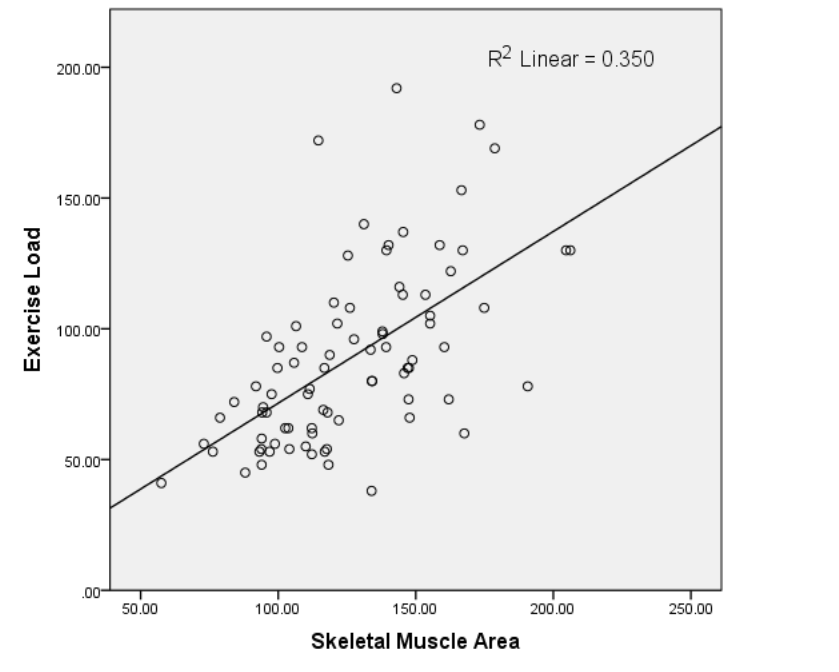
\includegraphics[width=\textwidth]{Figures/bc_scatter_pkLoad_skeletal}
		\caption{Peak Exercise}
		\label{fig:bc_pk_load_vs_sm}
	\end{subfigure}
	\caption{Correlation between exercise load and skeletal muscle area.}	
	\label{fig:bc_load_vs_sm}
	
\end{figure}

Exercise loads achieved at anaerobic threshold and at peak exercise capacity (at volitional stop rather than maximal exercise) were plotted against skeletal muscle area to create scatter-plots(Fig. \ref{fig:bc_load_vs_sm}, p\pageref{fig:bc_load_vs_sm}. 
Exercise load correlated positively with skeletal muscle area both at anaerobic threshold ($r^{2} = 0.284, p < 0.001$, Fig. \ref{fig:bc_at_load_vs_sm}) and at peak exercise ($r^{2} = 0.350, p < 0.001$, Fig. \ref{fig:bc_pk_load_vs_sm}). 
However, no correlation was identified between exercise loads achieved and adipose tissue area either at anaerobic threshold ($r^{2} = 0.004, p = 0.587$) or peak exercise ($r^{2} = 0.020, p = 0.206$) as shown in Table \ref{table:bc_cpet} on p\pageref{table:bc_cpet}. 

%This would suggest as one would expect that exercise capacity is mostly related to skeletal muscle volume rather than subcutaneous adipose tissue. - Move this to discussion 

\subsection{Body composition vs. oxygen consumption}

%Table 2
\begin{table}[p]
	\caption{The relationship between body composition and cardiopulmonary exercise testing controlled for sex in patients undergoing major pancreatic surgery.}
	\label{table:bc_cpet}
	\footnotesize
	\centering
	\renewcommand{\arraystretch}{1.5} %Increases space between rows
	%\setlength{\tabcolsep}{9pt} %sets the space between columns
	%\hline\noalign{\smallskip} %increases space after the line
	\begin{tabular}{|l| c c | c c | c c | c c|}
		\hline
		                          &  \multicolumn{2}{c|}{Subcut Fat}   & \multicolumn{2}{c|}{Visceral Fat}  &   \multicolumn{2}{c|}{Total Fat}   &    \multicolumn{2}{c|}{Skeletal}     \\
		                          & \multicolumn{2}{c|}{area (cm$^2$)} & \multicolumn{2}{c|}{area (cm$^2$)} & \multicolumn{2}{c|}{area (cm$^2$)} & \multicolumn{2}{c|}{muscle (cm$^2$)} \\
		Variable                  & $\rho$ & p                         & $\rho$ & p                         & $\rho$ & p                         & $\rho$ & p                           \\ \hline
		\multicolumn{9}{|c|}{Pulmonary Function Tests$^a$}                                                                                                                              \\ \hline
		FVC                       & -0.084 & 0.461                     & -0.111 & 0.332                     & -0.112 & 0.325                     & 0.303  & 0.007                       \\
		FEV1                      & -0.050 & 0.659                     & 0.043  & 0.704                     & -0.012 & 0.919                     & 0.350  & 0.002                       \\
		FEV1/FVC                  & 0.0    & 1.0                       & 0.200  & 0.077                     & 0.101  & 0.374                     & 0.003  & 978                         \\ \hline
		\multicolumn{9}{|c|}{At Rest$^b$}                                                                                                                                               \\ \hline
		Minute Ventilation        & 0.117  & 0.303                     & 0.076  & 0.504                     & 0.116  & 0.307                     & 0.136  & 0.230                       \\
		Tidal Volume              & 0.076  & 0.505                     & 0.130  & 0.252                     & 0.116  & 0.305                     & 0.301  & 0.007                       \\
		Absolute $\dot{V}_{O_2}$  & 0.123  & 0.277                     & 0.163  & 0.148                     & 0.164  & 0.145                     & 0.353  & 0.001                       \\
		Corrected $\dot{V}_{O_2}$ & -0.424 & $<$0.001                  & -0.396 & $<$0.001                  & -0.482 & $<$0.001                  & -0.194 & 0.085                       \\
		$O_2$ Pulse               & 0.110  & 0.330                     & 0.134  & 0.238                     & 0.141  & 0.212                     & 0.192  & 0.087                       \\ \hline
		\multicolumn{9}{|c|}{At Anaerobic Threshold$^b$}                                                                                                                                \\ \hline
		Exercise Load             & 0.085  & 0.454                     & 0.085  & 0.454                     & 0.105  & 0.349                     & 0.377  & 0.001                       \\
		Minute Ventilation        & 0.194  & 0.085                     & 0.127  & 0.261                     & 0.198  & 0.076                     & 0.263  & 0.018                       \\
		Tidal Volume              & 0.124  & 0.274                     & 0.154  & 0.172                     & 0.170  & 0.128                     & 0.436  & $<$0.001                    \\
		Absolute $\dot{V}_{O_2}$  & 0.191  & 0.089                     & 0.184  & 0.103                     & 0.231  & 0.038                     & 0.463  & $<$0.001                    \\
		Corrected $\dot{V}_{O_2}$ & -0.326 & 0.003                     & -0.365 & 0.001                     & -0.400 & $<$0.001                  & -0.078 & 0.487                       \\
		$O_2$ Pulse               & 0.181  & 0.108                     & 0.227  & 0.043                     & 0.242  & 0.029                     & 0.338  & 0.002                       \\ \hline
		\multicolumn{9}{|c|}{At Peak Exercise$^b$}                                                                                                                                      \\ \hline
		Exercise Load             & 0.029  & 0.799                     & -0.025 & 0.824                     & 0.020  & 0.859                     & 0.373  & 0.001                       \\
		Minute Ventilation        & 0.080  & 0.483                     & 0.080  & 0.483                     & 0.112  & 0.321                     & 0.242  & 0.029                       \\
		Tidal Volume              & 0.061  & 0.593                     & 0.153  & 0.174                     & 0.138  & 0.219                     & 0.409  & $<$0.001                    \\
		Absolute $\dot{V}_{O_2}$  & 0.087  & 0.444                     & 0.041  & 0.716                     & 0.093  & 0.407                     & 0.375  & 0.001                       \\
		Corrected $\dot{V}_{O_2}$ & -0.295 & 0.008                     & -0.365 & 0.001                     & -0.374 & 0.001                     & -0.027 & 0.813                       \\
		$O_2$ Pulse               & 0.200  & 0.075                     & 0.240  & 0.032                     & 0.261  & 0.019                     & 0.363  & 0.001                       \\ \hline
		\multicolumn{9}{l}{$\rho$ - Pearson's r adjusted for \textit{a} - age and sex and \textit{b} - sex.}
	\end{tabular}
\end{table}

Partial correlations between cardiopulmonary exercise parameters at rest, anaerobic threshold and peak exercise versus body composition were adjusted for gender. 
Our own findings (\ref{ch_cpet_jaundice}) and the findings of other authors suggest that age is not related to $\dot{V}_{O_2}$AT or $\dot{V}_{O_2}$Peak and therefore no adjustments were made for age. 
The results of this analysis are shown in Table \ref{table:bc_cpet} (p\pageref{table:bc_cpet}).

Tidal volume ($\dot{V}_T$, litres) was significantly correlated with skeletal muscle area at all phases of exercise including at rest, anaerobic threshold and peak exercise. 
There was a statistically significant but weak positive correlation between minute ventilation ($\dot{V}_E$, litres) and skeletal muscle at anaerobic threshold and peak exercise but not at rest. 
There was no correlation between either of these measures of pulmonary function and adipose tissue area at any phase of exercise.

%----------------------------------------------------------------------------------------------
% Correlation between body composition and $\dot{V}_{O_2}$AT before and after correction for total body weight.
\begin{figure}[htb]
	\centering
	\begin{subfigure}[b]{0.45\textwidth}
		\centering
		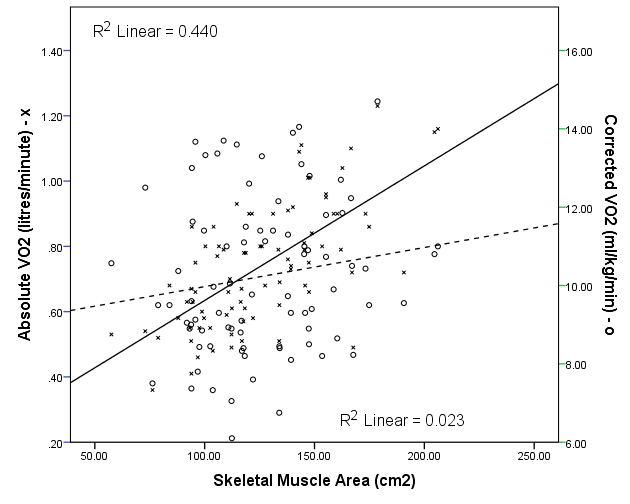
\includegraphics[width=\textwidth]{Figures/bc_scatter_VO2_skeletal}
		\caption{$\dot{V}_{O_2}$AT vs. 
Skeletal Muscle}
		\label{fig:bc_scatter_VO2_skeletal}
	\end{subfigure}
	\hfill
	\begin{subfigure}[b]{0.45\textwidth}
		\centering
		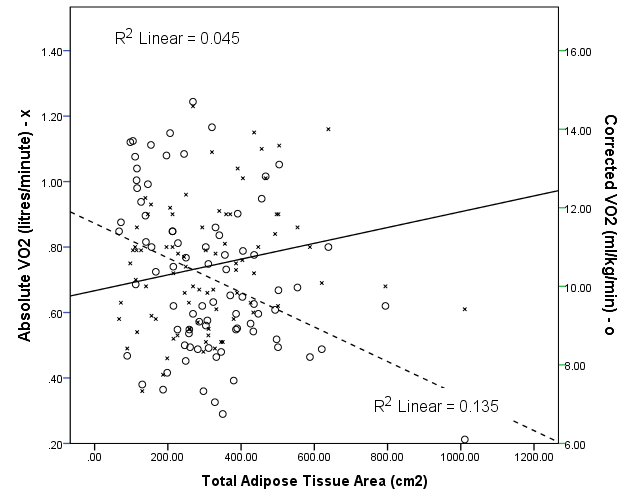
\includegraphics[width=\textwidth]{Figures/bc_scatter_VO2_TAT}
		\caption{$\dot{V}_{O_2}$AT vs. 
Total Adipose Tissue}
		\label{fig:bc_scatter_VO2_TAT}
	\end{subfigure}
	\caption{Correlation between body composition and $\dot{V}_{O_2}$AT before and after correction for total body weight.}	
	\label{fig:bc_scatter_VO2_bodycomp_reversal}
\end{figure}
%----------------------------------------------------------------------------------------------

Absolute $\dot{V}_{O_2}$ (litres/min) had a strong positive correlation with skeletal muscle area at rest ($\rho = 0.353, p = 0.001$), at anaerobic threshold ($\rho = 0.463, p<0.001$) and at peak exercise ($\rho = 0.375, p = 0.001$). 
However, this correlation was lost after correction of $\dot{V}_{O_2}$ for total body weight and in fact there was a non-significant change in the direction of correlation to the negative.

Absolute $\dot{V}_{O_2}$ (litres/min) had no correlation with total adipose tissue at rest or at peak exercise and only a weak correlation at anaerobic threshold. 
However, corrected for total body weight, there was a strong negative correlation between corrected $\dot{V}_{O_2}$ (ml/kg/min)and total adipose tissue at rest ($\rho = -0.482, p<0.001$), anaerobic threshold ($\rho = -0.400, p<0.001$) and peak exercise ($\rho = -0.374, p = 0.001$).

The loss of the physiological relationship between $\dot{V}_{O_2}$ and skeletal muscle after correcting for total body weight is shown in Fig.\ref{fig:bc_scatter_VO2_skeletal} and the creation of a spurious relationship with total adipose tissue after correction for total body weight is shown in Fig. \ref{fig:bc_scatter_VO2_TAT}.

$O_2$Pulse at the anaerobic threshold and peak exercise was strongly associated with skeletal muscle area with weaker positive correlations with visceral fat and total fat content. 
There was no correlation between $O_2$Pulse and subcutaneous adipose tissue at any phase of exercise.

%$\dot{V}_{O_2}$ corrected to height seems to correlate best with BC and everything else

\subsection{Scaling oxygen consumption to body composition and other factors}
Absolute $\dot{V}_{O_2}$ at the anaerobic threshold was corrected for weight, the square of height, body mass index, skeletal muscle area and estimated lean body mass. Calculation of estimated lean body mass is shown in Section \ref{sec:elbm}.
The resulting values were compared to body composition, height, weight and body mass index using partial correlations controlling for sex (Table \ref{table:bc_at_new_indices} on p\pageref{table:bc_at_new_indices}). 
The results from Table \ref{table:bc_cpet} comparing absolute $\dot{V}_{O_2}$ and corrected $\dot{V}_{O_2}$ at the anaerobic threshold with body composition are reproduced in the first two columns of this table to allow comparison with the new indices. 

$\dot{V}_{O_2}$ scaled for skeletal muscle area had no significant correlation with adipose tissue, height, weight or BMI but had a negative correlation with skeletal muscle area. 
$\dot{V}_{O_2}$ corrected for the square of patient's height had no correlation with adipose tissue but retained a positive correlation with skeletal muscle area as well as a positive correlation with total body weight and BMI. 

However, when absolute $\dot{V}_{O_2}$ was corrected for lean body mass, there was no correlation with any of the body composition indices or with height, weight or body mass index. 
The negative correlation between adipose tissue and $\dot{V}_{O_2}$ corrected for total body weight did not occur when $\dot{V}_{O_2}$ was corrected for lean body mass (Fig. \ref{fig:bc_scatter_VO2_TAT_elbm}). 
Moreover, the correlation with skeletal muscle area remained unchanged regardless of whether $\dot{V}_{O_2}$ was corrected for total body weight or lean body mass (Fig. \ref{fig:bc_scatter_VO2_skeletal_elbm}).

%----------------------------------------------------------------------------------------------
% Correlation between body composition and $\dot{V}_{O_2}$AT before and after correction for total body weight.
\begin{figure}[htb]
	\centering
	\begin{subfigure}[b]{0.45\textwidth}
		\centering
		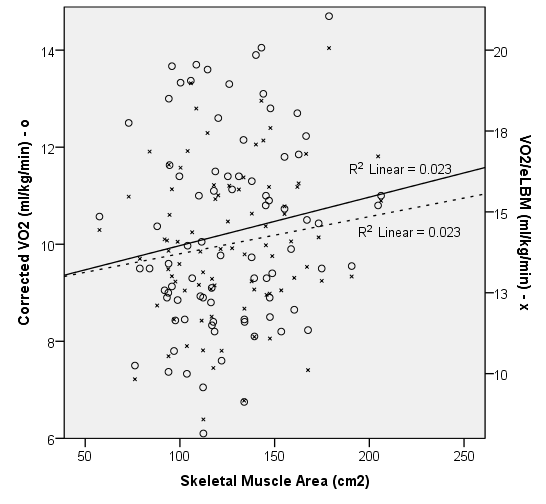
\includegraphics[width=\textwidth]{Figures/bc_scatter_VO2_skeletal_elbm}
		\caption{$\dot{V}_{O_2}$AT vs. 
Skeletal Muscle}
		\label{fig:bc_scatter_VO2_skeletal_elbm}
	\end{subfigure}
	\hfill
	\begin{subfigure}[b]{0.45\textwidth}
		\centering
		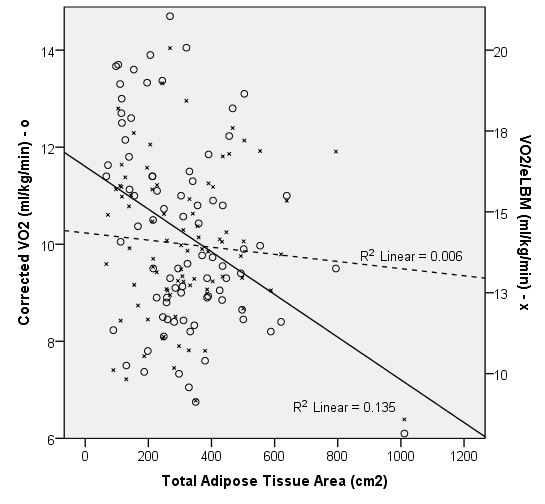
\includegraphics[width=\textwidth]{Figures/bc_scatter_VO2_TAT_elbm}
		\caption{$\dot{V}_{O_2}$AT vs. 
Total Adipose Tissue}
		\label{fig:bc_scatter_VO2_TAT_elbm}
	\end{subfigure}
	\caption{Correlation between body composition and $\dot{V}_{O_2}$AT corrected for total body weight and estimated lean body mass.}
	\label{fig:bc_scatter_VO2_bodycomp_elbm}
\end{figure}
%----------------------------------------------------------------------------------------------

\begin{sidewaystable}[p]
	\caption{The relationship between body composition, body habitus and $\dot{V}_{O_2}$AT scaled using different factors (controlled for sex) in patients undergoing major pancreatic surgery.}
	\label{table:bc_at_new_indices}
	\footnotesize
	\centering
	\renewcommand{\arraystretch}{1.5} %Increases space between rows
	%\setlength{\tabcolsep}{9pt} %sets the space between columns
	%\hline\noalign{\smallskip} %increases space after the line
	\begin{tabular}{|l|cc|cc|cc|cc|cc|cc|}
		\hline
		& \multicolumn{2}{c|}{Absolute $\dot{V}_{O_2}$} & \multicolumn{2}{c|}{$\frac{\dot{V}_{O_2}}{Weight}$} & \multicolumn{2}{c|}{$\frac{\dot{V}_{O_2}}{Height^2}$} & \multicolumn{2}{c|}{$\frac{\dot{V}_{O_2}}{BMI}$} & \multicolumn{2}{c|}{$\frac{\dot{V}_{O_2}}{Skeletal\ Muscle}$}  & \multicolumn{2}{c|}{$\frac{\dot{V}_{O_2}}{Lean\ Body\ Mass}$}\\
		
		Variable              	& $\rho$ &\textit{p}& $\rho$ &\textit{p}& $\rho$ &\textit{p}& $\rho$ &\textit{p}& $\rho$ &\textit{p}& $\rho$ &\textit{p} \\ \hline
		Subcut. fat (cm$^2$)     & 0.191  &  0.089   & -0.326 &  0.003   & 0.169  &  0.132   & -0.217 &  0.051   & 0.018  &  0.872   & -0.041 & 0.716 \\
		Visceral fat (cm$^2$)    & 0.184  &  0.103   & -0.365 &  0.001   & 0.154  &  0.168   & -0.279 &  0.012   & -0.065 &  0.563   & -0.108 & 0.339\\
		Total fat (cm$^2$)       & 0.231  &  0.038   & -0.400 & $<$0.001 & 0.191  &  0.088   & -0.286 &  0.010   & -0.021 &  0.851   & -0.082 & 0.466\\
		Skeletal Muscle (cm$^2$) & 0.463  & $<$0.001 & -0.078 &  0.487   & 0.329  &  0.003   & 0.105  &  0.353   & -0.429 & $<$0.001 & 0.133 & 0.237 \\
		Height (cm)               & 0.446  & $<$0.001 & 0.019  &  0.870   & 0.001  &  0.993   & 0.475  & $<$0.001 & 0.105  &  0.350   & 0.019 & 0.865\\
		Weight (kg)               & 0.545  & $<$0.001 & -0.302 &  0.006   & 0.358  &  0.001   & -0.043 &  0.703   & 0.001  &  0.995   & 0.033 & 0.770\\
		Body Mass Index (kg/m$^2$)      & 0.357  &  0.001   & -0.363 &  0.001   & 0.425  & $<$0.001 & -0.345 &  0.002   & -0.059 &  0.603   & 0.035 & 0.756\\ \hline
		\multicolumn{11}{l}{$\rho$ - Pearson's partial correlation adjusted for sex.}
	\end{tabular}
	\medskip
	\begin{flushleft}
		$\dot{V}_{O_2}$AT normalised using different measures of body habitus (including weight, square of height, body mass index, skeletal muscle area and estimated lean body mass) was compared to body composition as well as weight, height and BMI in an exploratory analysis. Scaling $\dot{V}_{O_2}$AT using estimated lean body mass was the only method studied that did not result in any 'spurious' correlations with body composition or body habitus. This is also depicted in Fig. \ref{fig:bc_scatter_VO2_bodycomp_elbm} on page \pageref{fig:bc_scatter_VO2_bodycomp_elbm}.
	\end{flushleft}
\end{sidewaystable}




\clearpage

\section{Discussion}

The results of this study demonstrate that the most important cardiopulmonary exercise test parameters used for preoperative risk evaluation in surgery are influenced significantly by the patient's body composition. 
Both $\dot{V}_{O_2}$AT and $\dot{V}_{O_2}$Peak were significantly affected by patient's body habitus when scaled using total body weight. 
Furthermore, the results suggest that there may be alternate methods of scaling of $\dot{V}_{O_2}$ that removes the effect of body composition on these parameters. 
The results also demonstrate the disproportionate decrease in skeletal muscle area with associated increase in adipose tissue with increasing body mass index. 

Taken together, these results would suggest that caution should be exercised in interpreting $\dot{V}_{O_2}$ (corrected for total body weight, ml/kg/min) in patients with a raised BMI.
Abnormally low values in these patients may not necessarily be due to poor aerobic fitness or lack of cardiopulmonary reserve and may simply be due to current convention used for scaling/representing $\dot{V}_{O_2}$.

\subsection{Oxygen consumption and body composition}

Increased physical activity such as during cardiopulmonary exercise testing or during and after surgery results in greater oxygen consumption ($\dot{V}_{O_2}$). 
The increased demand for oxygen is primarily due to increased metabolic activity within the exercising skeletal muscle.
Therefore, the positive correlation between absolute $\dot{V}_{O_2}$ and skeletal muscle area as has been found here is easily explained by the physiology of aerobic exercise. 

However, current convention is to report $\dot{V}_{O_2}$ measured at cardiopulmonary exercise testing according to the following formula: 
\[Corrected\ \dot{V}_{O_2} (ml.kg^{-1}.min^{-1}) = \frac{Absolute\ \dot{V}_{O_2}\ (litres.min^{-1}) * 1000}{Total\ body\ weight\ (kg)}\]

In chapter \ref{ch_cpet_jaundice}, we reported that there was a significant negative correlation between corrected $\dot{V}_{O_2}$ (ml/kg/min) and the patient's body mass index in spite of no observable cardiopulmonary comorbid disease (Tables \ref{table:cpet_oj_at_regression} and \ref{table:cpet_oj_peak_regression}). 
This negative correlation existed both at anaerobic threshold and peak exercise.
The results of the present study demonstrate that this negative correlation is consequent to the scaling convention used rather than due to any pathophysiological effect of obesity. 

The loss of the strong positive correlation between absolute $VO_{2}$ (litres/min) and skeletal muscle area after correcting for total body weight further supports the argument that the corrected value for $\dot{V}_{O_2}$ under-reports aerobic capacity in obese patients. 
There was no correlation between pulmonary function tests, tidal volume and minute ventilation and adipose tissue area as well as the slight.
However, a statistically significant, positive correlation was present between adipose tissue and $O_2$Pulse at anaerobic threshold as well as peak exercise but not at rest appear.
These findings suggest that adiposity did not contribute to poor cardiopulmonary exercise performance in this cohort of patients.

\subsection{Comparison with previous studies}
Our findings are similar to those reported by several authors previously. 
The relationship between body size, body composition and aerobic capacity both at rest and during exercise has been studied extensively for over a hundred years.

Seltzer reported in his 1940 study of 34 subjects, that individuals who were more `lateral' than `linear' had lower oxygen intakes per kilo body weight \parencite{seltzer_body_1940}.
Tanner in his article titled \textit{`Fallacy of per-weight and per-surface area standards, and their relation to spurious correlation'} in the Journal of Applied Physiology in 1947 recognised the dangers of expressing physiological variables as a function of total body mass \parencite{tanner_fallacy_1949}. 
In a detailed analysis comparing $\dot{V}_{O_2}$ and body build, he concluded that \textit{'as the index wt./stature increases, O2/wt. must be expected to decrease purely as a result of the method used for representing the data.'}

Batterham and co-workers studied 1314 apparently healthy men employed at the National Aeronautics and Space Administration Johnson Space Center in Houston, Texas \parencite{batterham_modeling_1999}. 
The authors reported that as body mass increased, the proportion composed of fat-free mass decreased. 
They also found that fat-free mass had a linear relationship with oxygen consumption while total body mass did not. 
They suggest that ideally estimates of fat-free mass should be used in the representation of oxygen consumption to allow more reliable comparison between subjects. 
These findings are similar to our results where the proportion of skeletal muscle area decreased significantly as body mass index increased with a greater decrease in females than males. 
Moreover, the linear relationship between skeletal muscle area and absolute $\dot{V}_{O_2}$ has also been clearly demonstrated in our findings. 

We used the Boer formula \parencite{boer_estimated_1984} to estimate lean body mass and used this to normalise $\dot{V}_{O_2}$. 
The resulting value for $\dot{V}_{O_2}$ showed no `spurious' correlations with body composition, height, total body weight or body mass index. 
These findings are similar to the recommendations made by Janz and co-workers who studied oxygen consumption and aerobic capacity in adolescents over several years as part of the Muscatine study and reported their findings in 1997 \parencite{janz_three-year_1997} and 1998 \parencite{janz_longitudinal_1998}. 
Aerobic capacity in the form of $\dot{V}_{O_2}$Peak was evaluated annually in 126 children (mean age 10.3 years) for five years. 
Body composition changes were also tracked over this period. 
They reported on the changes in body composition that occur over time and the differences in these changes between circum-pubertal boys and girls. 
They demonstrate significant difficulties in normalising $\dot{V}_{O_2}$ using total body mass and suggested that fat-free mass was the most appropriate variable for normalising $\dot{V}_{O_2}$. 
They found that $\dot{V}_{O_2}$ normalised using total body mass underestimated aerobic fitness levels of heavier boys and girls. 
However, this underestimation was greater in girls than in boys. 

In a study aimed at determining the optimal method of expressing $\dot{V}_{O_2}$Max, Maciejczyk and co-workers analysed the differing influence of body fat and lean body mass on aerobic performance in two groups of physically fit men categorised based on their body fat percentage \parencite{maciejczyk_influence_2014}. 
High body mass regardless of composition was correlated negatively with $\dot{V}_{O_2}$ (ml/kg/min) when it was corrected for total body weight penalising otherwise fit men purely based on the proportion of body weight that was contributed by body fat. 
However, when $\dot{V}_{O_2}$ was corrected for lean body mass, they found that the results were similar between the low body fat and high fat body groups. 
They, similar to Goran and co-workers \parencite{goran_total_2000}, recommend that $\dot{V}_{O_2}$ be normalised to lean body mass rather than total body weight.

Our results demonstrate that there is no correlation between absolute oxygen consumption at rest or during exercise and the amount of adipose tissue. 
This further emphasises the fact that adipose tissue is metabolically inactive during exercise although it contributes to increased work load. 
Therefore, dividing absolute $\dot{V}_{O_2}$ (l/min) by total body weight in overweight/obese subjects whose extra weight is largely due to adipose tissue would result in lower corrected $\dot{V}_{O_2}$ (ml/kg/min) as we have demonstrated here. 

Goran and co-workers reported that total body fat did not affect maximal aerobic capacity \parencite{goran_total_2000}. 
They reported on $\dot{V}_{O_2}$Max in obese women before and after weight loss. 
$\dot{V}_{O_2}$Max corrected for total body weight was significantly lower in obese subjects while $\dot{V}_{O_2}$Max corrected for fat-free mass did not change significantly after weight loss. 
They also reported that the limiting factor in obese patients was not the cardio-respiratory system but the fact that it was more difficult for obese individuals to do the same amount of work as a normal weight person in weight-bearing activities. 
This is likely due to the extra fat mass in these individuals that did not contribute to aerobic capacity but instead may have increased the exercise load in addition to that set by the investigator during the exercise.

These findings have been replicated by several other authors in different subject groups \parencite{loftin_scaling_2001, lemaitre_maximum_2006, savonen_current_2012, krachler_cardiopulmonary_2014}. 
Several of the above studies also recommended using allometric scaling to avoid the confounding effects of total body weight. 
However, this has not gained widespread clinical use.

The conclusion from the above studies would be that oxygen consumption normalised for total body weight unfairly penalises obese patients in the absence of true impairment of cardio-respiratory function. 
This has significant clinical implications as outlined below.

\subsection{Clinical implications of spurious correlation}

The term \textit{`spurious correlation'} was first introduced by English mathematician and biometrician, Karl Pearson in 1896. 
He used the term to describe correlations that occurred as a result of using ratios instead of absolute values rather than because of any actual correlations between the variables being studied \parencite{pearson_mathematical_1896}.

Older and co-workers in their pioneering study in 1993 reported that $\dot{V}_{O_2}$AT $<$ 11 ml/kg/min was associated with increased mortality in elderly patients undergoing major abdominal surgery \parencite{older_preoperative_1993}. 
While they did not provide any data on other preoperative or intra-operative factors, they concluded that cardiopulmonary exercise testing was useful in predicting postoperative outcome and that a low $\dot{V}_{O_2}$AT represented cardiac failure. 
This association is repeated in their later work on 548 patients which also showed a clear association between low $\dot{V}_{O_2}$AT (ml/kg/min) and mortality due to cardiovascular causes \parencite{older_cardiopulmonary_1999}. 
The concepts of \textit{'surgical anaerobic threshold'} and \textit{'postoperative cardiac failure'} were introduced later and were described as the \textit{'inability of the heart to meet the demand of postoperative stress.'}\parencite{society_ats/accp_2003}.

Swart and Carlisle als reported that $\dot{V}_{O_2}$AT $<$ 11 ml/kg/min in patients undergoing open colorectal surgery was associated with adverse outcomes \parencite{swart_case-controlled_2012}. 
However, the proportion of females in the low $\dot{V}_{O_2}$AT group was significantly greater than that in the normal $\dot{V}_{O_2}$AT group (24\% vs 51\%). 
The average corrected $\dot{V}_{O_2}$AT in men calculated from the data presented in their paper was 11.02 ml/kg/min while in women it was 9.81 ml/kg/min. 

In a study by Wilson and co-workers which reported that cardiopulmonary exercise testing predicted outcome after major elective intra-abdominal surgery, the proportion of females in the low $\dot{V}_{O_2}$AT group was 51\% while it was 28\% in the group with normal AT \parencite{wilson_impaired_2010}. 
There was no data presented on body mass index in this study. 
We reported in Chapter \ref{ch_cpet_jaundice} that females were more likely to have a lower $\dot{V}_{O_2}$AT (Table \ref{table:cpet_oj_at_regression}) and lower $\dot{V}_{O_2}$Peak (Table \ref{table:cpet_oj_peak_regression}). 
However, all the results in the present study were controlled for the effect of sex. 

The `obesity paradox' would suggest that, in fact, obese patients are not necessarily at an increased risk of postoperative complications. 
Several authors have reported that obesity is not a risk factor for major complications after pancreaticoduodenectomy \parencite{khan_does_2010, tsai_impact_2010, balentine_obesity_2011}. 
In a large study of 118,707 patients undergoing non-bariatric general surgery, the authors reported that the risk of death was `paradoxically' low in the overweight and obese group of patients \parencite{mullen_obesity_2009}. 
The results of the present study show that $\dot{V}_{O_2}$ as is currently reported for clinical use will also be low in this very same cohort of patients. 
This obesity paradox is particularly apparent in patients with heart failure where in spite of a low $\dot{V}_{O_2}$ (corrected for total body weight), obese patients have better survival rates. 
Horwich and co-workers reported in a study of 2331 patients that body mass index was associated with a low $\dot{V}_{O_2}$Peak (ml/kg/min) independent of all other factors including age, diabetes, cardiac disease, New York Heart Association Class of cardiac failure and race \parencite{horwich_relationship_2009}.

It is clear from the review presented in Chapter \ref{ch_intro} as well as the results presented in Chapter \ref{ch_cpet_outcomes}, that cardiopulmonary exercise testing is useful in predicting risk after major surgery. 
Cardiopulmonary exercise testing has become ubiquitous in the preoperative assessment of complex surgical patients. 
However, the present study demonstrates that cardiopulmonary exercise test parameters in the overweight/obese patient must be interpreted with caution, especially when used to select patients who may be declined surgery based on these results. 

\subsection{Measuring impact of prehabilitation}

Where time to surgery is not critical, prehabilitation has gained an increasingly important role in optimising patients for surgery.
Prehabilitation has been defined as the `process of enhancing functional capacity of the individual to enable him or her to withstand the stressor of inactivity' \parencite{topp_effect_2002}. 
Jones and co-workers reported an increase in $\dot{V}_{O_2}$Peak by an average 2.4 ml/kg/min when patients were placed on an aerobic exercise regimen before undergoing surgery for lung cancer \parencite{jones_effects_2007}. 
Kim and co-workers also demonstrated a significant improvement in exercise loads achieved as well as sub-maximal oxygen consumption in patients who undertook a 4-week exercise program before major bowel surgery \parencite{kim_responsive_2009}.
Moreover, deterioration in aerobic capacity during prehabilitation was reported to be associated with increased incidence of postoperative complications \parencite{mayo_impact_2011}. 

However, other authors have not been able to reproduce these findings. 
Patient compliance and difficulties in trying to modify lifestyle prior to surgery were considered important factors for failure of prehabilitation \parencite{carli_randomized_2010, dronkers_preoperative_2010}.

Cardiopulmonary exercise testing has been reported to be a useful objective measure of the impact of prehabilitation in surgical patients. 
It was used to demonstrate the decline in $\dot{V}_{O_2}$AT associated with neo-adjuvant chemoradiotherapy in patients with rectal cancer who did not undertake an exercise program.
However, $\dot{V}_{O_2}$AT improved in the intervention group who undertook a 6 week exercise program \parencite{west_effect_2015}.

However, the results presented in this study demonstrate that the success of such prehabilitation programs must not be determined solely by $\dot{V}_{O_2}$ corrected for total body weight. 
Instead, improvement in the absolute values of $\dot{V}_{O_2}$AT and $\dot{V}_{O_2}$Peak in conjunction with improvement in other parameters that are not affected by body composition such as $O^2$Pulse, tidal volume \parencite{jones_effects_2007} or maximal exercise load \parencite{kim_responsive_2009} may provide more reliable evidence of improvement in aerobic capacity. 

The combination of nutritional assessment and advice, home-based exercise programs and weight loss may help improve aerobic capacity and eventually postoperative outcomes. 
Such preoperative interventions may also be associated with improvements in body composition with increase in skeletal muscle mass and reduction in adipose tissue.
This may result in apparent improvements in cardiopulmonary exercise test parameters that are scaled using total body weight.
Further studies are required to validate the findings presented here as well as to identify optimal scaling methods for cardiopulmonary exercise test parameters. 
This will improve the clinical utility of cardiopulmonary exercise testing in the preoperative risk assessment as well as optimisation of patients undergoing major surgery.
